
  \chapter{Schemat działania projektu}
    Do sprawnej wymiany informacji między urządzeniami potrzebne jest kilka tematów. Oprogramowanie służące do trzymania piecza nad tymi drogami komunikacji działa tak że w razie potrzeby automatycznie potrafi tworzyć niezbędne tematy, dzięki czemu niezależnie czy dany broker już wcześniej obsługiwał to urządzenia czy nie, system potrafi samodzielnie przygotować sobie środowisko pracy.
    
    \vspace{1em} 
    Tematy tworzone i zarządzane przez aplikację okienkową to:

    \begin{itemize}
      \item kp - Wartość członu proporcjonalnego. Parametr sterujący pracą regulatora PID,
      \item ki - Wartość członu całkującego. Parametr sterujący pracą regulatora PID,
      \item kd - Wartość członu różniczkującego. Parametr sterujący pracą regulatora PID, 
      \item setpoint - Wartość zadana dla regulatora. Wyrażona w obrotach na minutę. 
    \end{itemize}

    Należy zauważyć że są to tylko i wyłącznie wartości zarządzające pracą regulatora PID. Dzięki udostępnieniu ich poza obszar programu istnieje możliwość dynamicznej zmiany parametrów regulatora, co sprawia że nawet osoba nie mająca dużego doświadczenia z regulatorami PID potrafi empirycznie wyznaczyć zadowalające wartości. 
    
    \vspace{1em} 
    Poza tematami utworzonymi przez aplikację dostępową, potrzebne są jeszcze trzy dodatkowe tematy:

    \begin{itemize}
      \item rpm - ilość obrotów odczytana z silnika przy pomocy enkodera. Wyrażona w obrotach na minutę. Służy jedynie w celach kontrolnych. Daje możliwość zorientować się z jaką prędkością obraca się silnik w rzeczywistości i porównać wynik z wartością zadaną.
      \item pwm\_duty - wartość wypełnienia PWM, wyrażona w procentach. Obrazuje stopień wykorzystania silnika.
      \item voltage - Napięcie zasilania urządzenia. Według specyfikacji L298 napięcie dostarczane do silników jest niższe o 1.8V - 3.2V w zależności od obciążenia. \cite{mostek}
    \end{itemize}
    
    Obaj klienci brokera MQTT subskrybują nawzajem swoje tematy. Schemat wymiany danych został przedstawiony na rysunku \ref{data_transmision}. Obrazuje on sposób komunikacji i zależności.
    
    \begin{figure}[ht]
      \centering
      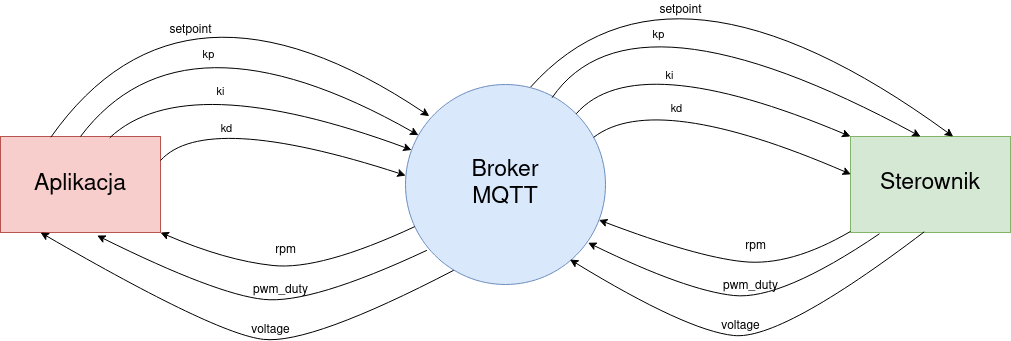
\includegraphics[width=1\textwidth]{img/dane.png}
      \caption{Schemat wymiany danych w systemie}
      \label{data_transmision}
    \end{figure}
